\section{Erinnerung und Beispiele}

\begin{erinnerung}
	\proplbl{1_1_1}
	Eine \begriff{Gruppe} ist ein Paar $(G,\ast)$ bestehend aus einer Menge $G$ und einer Verknüpfung $\ast: G\times G\to G$, dass die Axiome Assoziativität, Existenz eines neutralen Elements und Existenz von Inversen erfüllt, und wir schreiben auch $G$ für die Gruppe $(G,\ast)$. Die Gruppe $G$ ist \begriff[Gruppe!]{abelsch}, wenn $g\ast h=h\ast g$ für alle $g,h\in G$. Eine allgemeine Gruppe schreiben wir multiplikativ mit neutralem Element 1, abelsche Gruppen auch additiv mit neutralem Element 0.
	
	Eine Teilmenge $H\subseteq G$ ist eine \begriff{Untergruppe} von $G$, in Zeichen $H\le G$, wenn $H\neq\emptyset$ und $H$ abgeschlossen ist unter der Verknüpfung und den Bilden von Inversen. Wir schreiben 1 (bzw. 0) auch für die triviale Untergruppe $\{1\}$ (bzw. $\{0\}$) von $G$.
	
	Eine Abbildung $\phi:G\to G'$ zwischen Gruppen ist ein \begriff{Gruppenhomomorphismus}, wenn
	\begin{align}
		\phi(g_1\cdot g_2) = \phi(g_1)\cdot\phi(g_2)\quad\forall g_1,g_2\in G\notag
	\end{align}
	und in diesem Fall ist 
	\begin{align}
		\Ker(\phi) = \phi^{-1}(\{1\})\notag
	\end{align}
	der \begriff{Kern} von $\phi$. Wir schreiben $\Hom(G,G')$ für die Menge der Gruppenhomomorphismen $\phi:G\to G'$.
\end{erinnerung}

\begin{example}
	Sei $n\in\natur$, $K$ ein Körper und $X$ eine Menge.
	\begin{enumerate}[label=(\alph*)]
		\item $\Sym(X)$, die \begriff{symmetrische Gruppe} aller Permutationen der Menge $X$ mit $f\cdot g=g\circ f$, insbesondere $S_n=\Sym(\{1,...,n\})$
		\item $\whole$ sowie $\whole/n\whole=\{a+n\whole\mid a\in\whole\}$ mit der Addition
		\item $\GL_n(K)$ mit der Matrizenmultiplikation, Spezialfall $\GL_1(K)=K^\times=K\backslash\{0\}$
		\item Für jeden Ring $R$ bilden die Einheiten $R^\times$ eine Gruppe unter der Multiplikation, zum Beispiel $\Mat_n(K)^\times=\GL_n(K)$, $\whole^\times=\mu_2=\{1,-1\}$
	\end{enumerate}
\end{example}

\begin{example}
	Ist $(G,\cdot)$ eine Gruppe, so ist auch $(G^{op},\cdot^{op})$ mit $G=G^{op}$ und $g\cdot^{op}h=h\cdot g$ eine Gruppe.
\end{example}

\begin{remark}
	\proplbl{1_1_4}
	Ist $G$ eine Gruppe und $h\in G$, so ist die Abbildung
	\begin{align}
		\tau_h=\begin{cases}
			G\to G \\ g\mapsto gh
		\end{cases}\notag
	\end{align}
	eine Bijektion (also $\tau_h\in\Sym(G)$) mit Umkehrabbildung $\tau_{h^{-1}}$.
\end{remark}

\begin{proposition}
	Sei $G$ eine Gruppe. Zu jeder Menge $X\subseteq G$ gibt es eine kleinste Untergruppe $\langle X\rangle$ von $G$, die $X$ enthält, nämlich
	\begin{align}
		\langle X\rangle = \bigcap_{X\subseteq H\le G} H\notag
	\end{align} 
\end{proposition}

\begin{remark}
	Man nennt $\langle X\rangle$ die von $X$ \begriff[Untergruppe!]{erzeugte} von $G$. Die Gruppe $G$ heißt \begriff[Gruppe!]{endlich erzeugt}, wenn $G=\langle X\rangle$ für eine endliche Menge $X\subseteq G$.
\end{remark}

\begin{proposition}
	Ein Gruppenhomomorphismus $\phi:G\to G'$ ist genau dann ein Isomorphismus, wenn es einen Gruppenhomomorphismus $\phi':G'\to G$ mit $\phi'\circ\phi=\id_G$ und $\phi\circ\phi'=\id_{G'}$ gibt.
\end{proposition}

\begin{example}
	Ist $G$ eine Gruppe, so bilden die \begriff{Automorphismen} $\Aut(G)\subseteq\Hom(G,G)$ eine Gruppe unter $\phi\circ\phi'=\phi'\circ\phi$. Für $\phi\in\Aut(G)$ und $g\in G$ schreiben wir $g^\phi=\phi(g)$.
\end{example}

\begin{proposition}
	Einen Gruppenhomomorphismus $\phi:G\to G'$ ist genau dann injektiv, wenn $\Ker(\phi)=1$.
\end{proposition}

\begin{example}
	Sei $n\in\natur$, $K$ ein Körper.
	\begin{enumerate}[label=(\alph*)]
		\item $\sgn:S_n\to\mu_2$ ist ein Gruppenhomomorphismus mit Kern die \begriff{alternierende Gruppe} $A_n$.
		\item $\det:\GL_n(K)\to K^\times$ ist ein Gruppenhomomorphismus mit Kern $\SL_n(K)$.
		\item $\pi_{n\whole}:\whole\to\whole/n\whole$, $a\mapsto a+n\whole$ ist ein Gruppenhomomorphismus mit Kern $n\whole$
		\item Ist $A$ eine abelsche Gruppe, so ist
		\begin{align}
			[n]:\begin{cases}
				A\to A \\ x\to nx
			\end{cases}\notag
		\end{align}
		ein Gruppenhomomorphismus mit Kern $A[n]$, die $n$-Torsion von $A$ und Bild $nA$.
		\item Ist $G$ eine Gruppe, so ist
		\begin{align}
			\begin{cases}
				G\to G^{op} \\ g\mapsto g^{-1}
			\end{cases}\notag
		\end{align}
		ein Isomorphismus.
	\end{enumerate}
\end{example}

\begin{definition}[Zykel, disjunkte Zykel]
	\proplbl{1_1_11}
	Seien $n,k\in\natur$. Für paarweise verschiedene Elemente $i_1,...,i_k\in\{1,...,n\}$ bezeichnen wir mit $(i_1...i_k)$ das $\sigma\in S_n$ gegeben durch
	\begin{align}
		\sigma(i_j) &= i_{j+1} \quad \text{für } j=1,...,k-1 \notag \\
		\sigma(i_k) &= i_1 \notag \\
		\sigma(i) &= i \quad \text{für } i\in\{1,...,n\}\backslash\{i_1,...,i_k\}\notag
	\end{align}
	Wir nennen $(i_1...i_k)$ eine $k$-\begriff{Zykel}. Zwei Zykel $(i_1...i_k)$ und $(j_1...j_l)\in S_n$ heißen \begriff[Zykel!]{disjunkt}, wenn $\{i_1,...,i_k\}\cap\{j_1,...,j_l\}=\emptyset$.
\end{definition}

\begin{proposition}
	Jedes $\sigma\in S_n$ ist das Produkt von Transpositionen (das heißt 2-Zykeln).
\end{proposition}

\begin{lemma}
	Disjunkte Zykel kommutieren, das heißt sind $\tau_1,\tau_2\in S_n$ disjunkte Zykel, so ist $\tau_1\tau_2 = \tau_2\tau_1$.
\end{lemma}
\begin{proof}
	Sind $\tau_1=(i_1...i_k)$ und $\tau_2=(j_1...j_l)$ so ist
	\begin{align}
		\tau_1\tau_2(i)=\tau_2\tau_1(i)=\begin{cases}
			\tau_1(i) & i\in\{i_1...i_k\} \\
			\tau_2(i) & i\in\{j_1...j_l\} \\
			i & \text{sonst}
		\end{cases}\notag
	\end{align}
\end{proof}

\begin{proposition}
	Jedes $\sigma\in S_n$ ist ein Produkt von paarweise disjunkten $k$-Zykeln mit $k\ge 2$ eindeutig bis auf Reihenfolge (sogenannte \begriff{Zykelzerlegung} von $\sigma$). 
	\begin{center}
		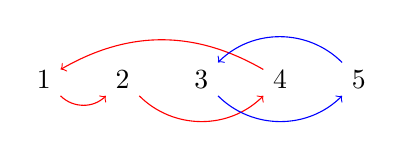
\begin{tikzpicture}
			\node at (0,0) (1) {1};
			\node at (1,0) (2) {2};
			\node at (2,0) (3) {3};
			\node at (3,0) (4) {4};
			\node at (4,0) (5) {5};
			
			\draw[red,->] (1) to [bend right=45] (2);
			\draw[red,->] (2) to [bend right=45] (4);
			\draw[red,->] (4) to [bend right=30] (1);
			
			\draw[blue,->] (3) to [bend right=45] (5);
			\draw[blue,->] (5) to [bend right=45] (3);
		\end{tikzpicture}
	\end{center}
	Also ein \textcolor{red}{3-Zykel} und ein \textcolor{blue}{2-Zykel}.
\end{proposition}
\begin{proof}
	Induktion nach $N=\vert \{i\mid \sigma(i)\neq i\}\vert$. \\
	\emph{$N=0$:} $\sigma=\id$ \\
	\emph{$N>0$:} Wähle $i_1$ mit $\sigma(i_1)\neq i_1$, betrachte $i_1,\sigma(i_1),\sigma^2(i_1),...$. Da $\{1,...,n\}$ endlich und $\sigma$ bijektiv ist, existiert ein minimales $k\ge 2$ mit $\sigma^k(i_1)=i_1$. Setze $\tau_1=(i_1\,\sigma(i_1)...\sigma^{k-1}(i_1))$. Dann ist $\sigma=\tau_1\circ\tau_1^{-1}\sigma$, und nach Induktionshypothese ist $\tau_1^{-1}\sigma=\tau_2\circ...\circ\tau_m$ mit disjunkten Zyklen $\tau_2,...,\tau_m$. \\
	Eindeutigkeit ist klar, denn jedes $i$ kann nur in einem Zykel $(i\,\sigma(i)...\sigma^{k-1}(i))$ vorkommen.
\end{proof}

\begin{*example}
	$(1\, 2\, 3\, 4\, 5)(2\, 4)=(1\, 4\, 5)(2\, 3)=(2\, 3)(1\, 4\, 5)=(3\, 2)(1\, 4\, 5)=(3\, 2)(4\, 5\, 1)\neq (3\, 2)(1\, 5\, 4)$
\end{*example}
